\documentclass[11pt,a4paper]{article}
\usepackage[utf8]{inputenc}
\usepackage[english]{babel}
\usepackage{amsmath}
\usepackage{amsfonts}
\usepackage{amssymb}
\usepackage{graphicx}
\usepackage[left=2cm,right=2cm,top=2cm,bottom=2cm]{geometry}
\begin{document}

\begin{flushright}
BIOS 6643 Fall 2021

Homework 1

Ian Arriaga MacKenzie
\end{flushright}

\textbf{Question 1}\\

I have read and agree to the homework expectations.\\

\textbf{Question 2}\\

\textit{(a)}\\

Performing a linear regression of the change-score on the intercept yields the mean: -19.54 (95\% CI: -26.63, -12.44; p-value: 8.43E-6).\\

\textit{(b)}\\

The t-test for a mean of 0 yields the same results.\\

\textit{(c)}\\

The results for the baseline-as-covariate model is:

\begin{table}[ht]
\centering
\begin{tabular}{c|c|c|c|c|}
\cline{2-5}
                                & Estimate & 2.5\% CI & 97.5\% CI & P-value \\ \hline
\multicolumn{1}{|c|}{Intercept} & 37.15    & 2.85     & 71.45     & 0.035   \\ \hline
\multicolumn{1}{|c|}{Baseline}  & 0.69     & 0.51     & 0.87      & 5.39E-8 \\ \hline
\end{tabular}
\end{table}

\textit{(d)}\\

The change score model is just the t-test for a mean of 0, whereas the baseline-as-covariate model is a true linear model with a slope over the parameter of interest. We can see this from the residuals as well:

\begin{center}
CS Model

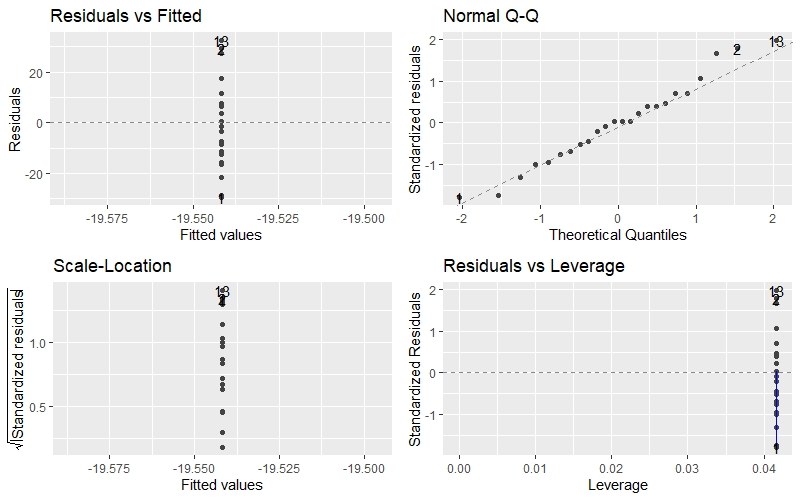
\includegraphics[scale = 0.7]{cs_model_resid.jpeg}
\end{center}

\begin{center}
BAC Model

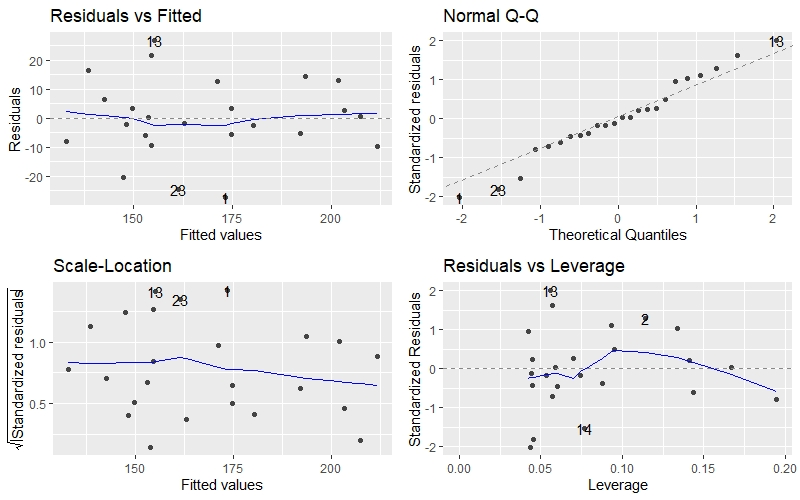
\includegraphics[scale = 0.7]{bs_model_resid.jpeg}
\end{center}

\textit{(e)}\\

The results for the hybrid model are:

\begin{table}[ht]
\centering
\begin{tabular}{c|c|c|c|c|}
\cline{2-5}
                                & Estimate & 2.5\% CI & 97.5\% CI & P-value \\ \hline
\multicolumn{1}{|c|}{Intercept} & 37.15    & 2.85     & 71.45     & 0.035   \\ \hline
\multicolumn{1}{|c|}{Baseline}  & -0.30    & -0.48    & -0.12     & 0.00213 \\ \hline
\end{tabular}
\end{table}

Which can be expressed as:

$$ Y_{Change Score} = \beta_0 + \beta_1 \cdot X_{Baseline} $$

$$ X_{Baseline} = \dfrac{Y_{Change Score} - \beta_0}{\beta_1} $$

The Hybrid and BAC models are the same in that they have the same intercept $\beta_0$, but differing slopes on the baseline. The hypothesis of interest is:

$$ H_0 : \beta_1 = 0 \hspace{2cm} H_1 : \beta_1 \neq 0 $$

\textit{(f)}\\

I tried to fit a linear mixed effects model, but it kept regressing to the original Hybrid linear model as there were no repeated measures in the data. We return a singular fit matrix, and the estimates are the same as above.\\

\textbf{Question 3}\\

\textit{(a)}

$$ E [ \epsilon_t ] = E \left[ \sum_{j=0}^k \phi^j Z_{t-j} \right] = \sum_{j=0}^k \phi^j \left( E \left[ Z_{t-j} \right] \right) = \sum_{j=0}^k \phi^j \left( 0 \right) = 0$$

\newpage
\textit{(b)}

$$ Cov [ \epsilon_t, \epsilon_{t+h} ] = E [ \epsilon_t \epsilon_{t+h} ] - E [ \epsilon_t ] E [ \epsilon_{t+h} ] = E [ \epsilon_t \epsilon_{t+h} ] $$

$$ \epsilon_{t+h} = \phi \epsilon_t + Z_{t+h} \Rightarrow E [ \epsilon_t \epsilon_{t+h} ] = E [ \epsilon_t \left( \phi \epsilon_t + Z_{t+h} \right) ] = E [ \phi \epsilon_t^2 + Z_{t+h} \epsilon_t ] = \phi E [ \epsilon_t^2 ] + E [ Z_{t+h} \epsilon_t ] $$

$$ Z_{t+h} \bot Z_{t-j} \Rightarrow E [ Z_{t+h} \epsilon_t ] = E \left[ Z_{t+h} \sum_{j=0}^k \phi^j Z_{t-j} \right] = E [ Z_{t+h} ] E \left[ \sum_{j=0}^k \phi^j Z_{t-j} \right] = 0 $$

$$ Var [ e_t ] = E [ e_t^2 ] - E [ e_t ]^2 = E [ e_t^2 ] \Rightarrow \phi E [ e_t^2 ] = \phi Var [e_t] $$

$$ Var [e_t] = Var \left[ \sum_{j=0}^k \phi^j Z_{t-j} \right] = \sum_{j=0}^k \phi^{2j} Var [ Z_{t-j} ] =  \sum_{j=0}^k \phi^{2j} \sigma^2 = \sigma^2  \underbrace{\sum_{j=0}^k \phi^{2j}} = \dfrac{\sigma^2}{1 - \phi^2} $$

\hspace{11cm} Geometric Series

$$ Cov [ \epsilon_t, \epsilon_{t+h} ] = \dfrac{\phi \sigma^2}{1 - \phi^2} $$

\textit{(c)}

$$ Corr [ \epsilon_t, \epsilon_{t+h} ] = \dfrac{Cov [ \epsilon_t, \epsilon_{t+h} ]}{\sigma_t \cdot \sigma_{t+h}} = \dfrac{Cov [ \epsilon_t, \epsilon_{t+h} ]}{\sqrt{ Var [ e_t ] } \sqrt{ Var [ e_{t+h} ] }} = \dfrac{\dfrac{\phi \sigma^2}{1 - \phi^2}}{\sqrt{\dfrac{\sigma^2}{1 - \phi^2}} \sqrt{\dfrac{\sigma^2}{1 - \phi^2}}} = \phi $$

\textit{(d)}\\

Yes $\lbrace e_t \rbrace $ is a stationary process. The expectation is 0 and therefor constant. The autocovariance function is also finite, and so this is has weak-sense stationarity.\\

\newpage
\textbf{Question 4}\\

\textit{(a)}\\

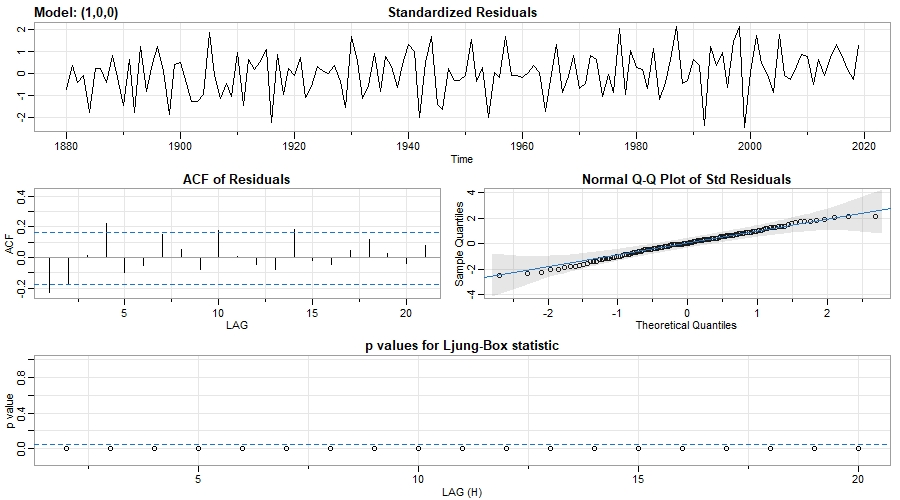
\includegraphics[width=\textwidth]{time_resid_1.jpeg}

Looking at the residuals we see roughly equal variance across the time series, however we do see a slight trend upward over time instead of a mean of 0 across the sample. The residuals are normal, however the autocorrelation function and Ljung-Box statistic show that our model could be fit better.\\

\textit{(b)}

\begin{center}
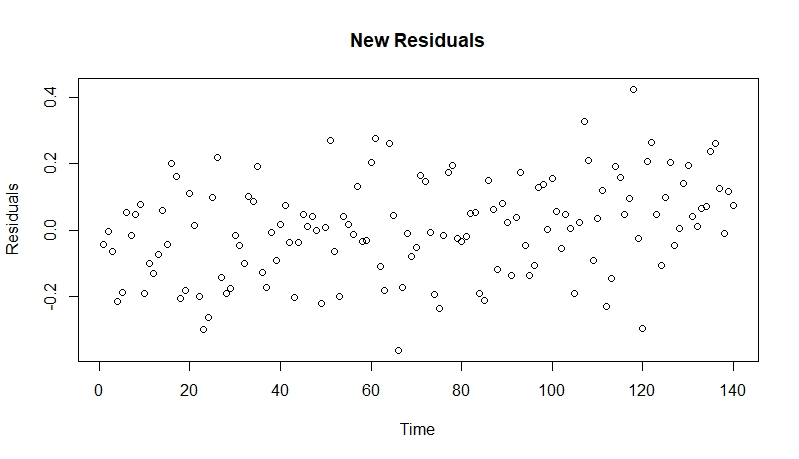
\includegraphics[scale = 0.8]{newres_ar1.jpeg}
\end{center}

Here we see the residuals have centered around 0 more, and the upward trend in time has decreased slightly.\\

\textit{(c)}\\

Fitting the AR(1) time series model, we get the covariates:

\begin{table}[ht]
\centering
\begin{tabular}{c|c|c|}
\cline{2-3}
                                 & ar1    & xmean  \\ \hline
\multicolumn{1}{|c|}{Estimate}   & 0.9484 & 0.1411 \\ \hline
\multicolumn{1}{|c|}{Std. Error} & 0.0286 & 0.1795 \\ \hline
\end{tabular}
\end{table}

Which gives us the model:

$$ x_t = 0.1411 - ( 0.1411 \cdot 0.9484) + 0.9484 \cdot x_{t-1} + w_t = 0.00728 + 0.9484 \cdot x_{t-1} + w_t $$

and the increase per decade would be:

$$ \dfrac{0.9484}{\mbox{14 Decades} } = 0.0677 \mbox{ Degrees per Decade} $$

\textit{(d)}\\

Fitting a linear model with a polynomial trend for time yields a slightly better fitting model by LL/AIC:

\begin{table}[ht]
\centering
\begin{tabular}{c|c|c|}
\cline{2-3}
                                      & Log Likelihood & AIC     \\ \hline
\multicolumn{1}{|c|}{AR(1)}           & 96.05          & -186.11 \\ \hline
\multicolumn{1}{|c|}{Polynomial Time} & 110.91         & -209.83 \\ \hline
\end{tabular}
\end{table}

And examining the residuals yields no obvious problems aside from some slight heteroscedasticity:\\

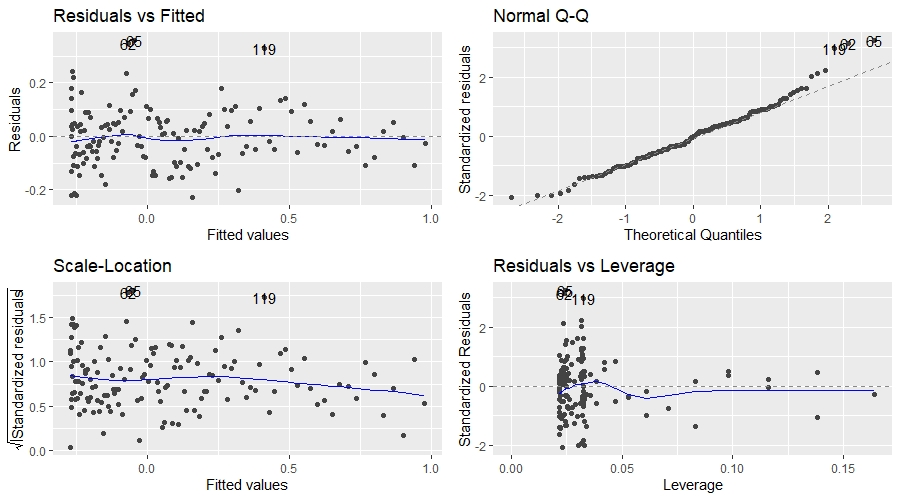
\includegraphics[width=\textwidth]{poly_resid_4d.jpeg}

\textit{(e)}\\

Fitting a LOESS model:\\

\begin{center}
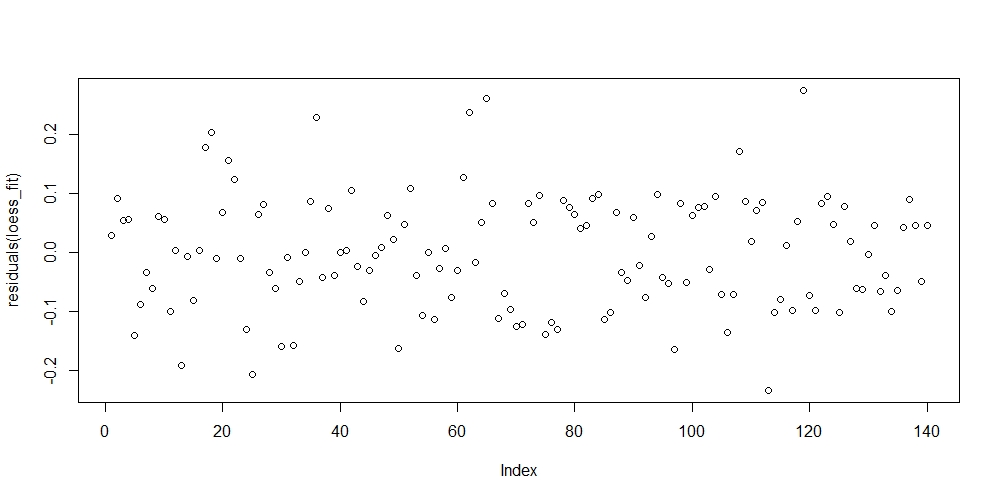
\includegraphics[scale = 0.4]{resid_loess.jpeg}
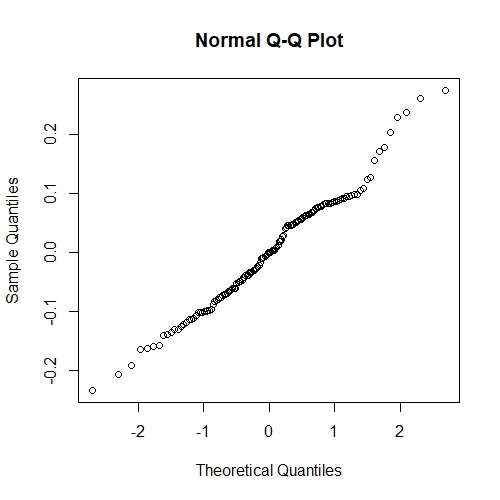
\includegraphics[scale = 0.4]{qq_loess.jpeg}
\end{center}

The residuals and Q-Q plot look good, and the fit seems to indicate an upward trend in time:

\begin{center}
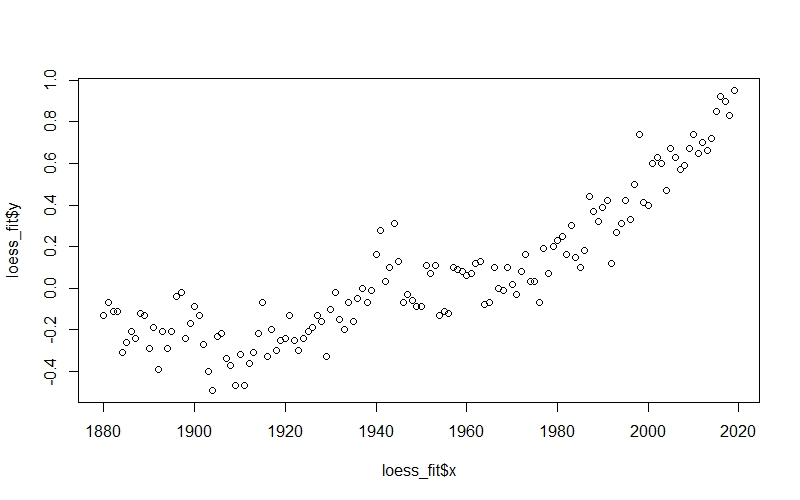
\includegraphics[scale = 0.8]{loess_fit.jpeg}
\end{center}

Based on the diagnostic plots, either the polynomial model or loess model would be adequate, however I would not use the AR(1) model for this data.



\end{document}